\chapter{Zadanie 2.}
Zar�wno sterowanie, jak i zak��cenie zosta�y wzbudzone do warto?ci:
\begin{itemize}
\item {\color{green}$ \num{0.8} $}
\item {\color{red}$ \num{0.4} $}
\item {\color{blue}$ \num{-0.4} $}
\item {\color{purple}$ \num{-0.8} $}
\end{itemize}

Odpowiedzi skokowe dla toru wej�cie-wyj�cie wida� na rysunku ~\ref{odp_skok_u} a dla toru zak��cenie wyj�cie na rysunku ~\ref{odp_skok_z}.

\begin{figure}[b]
\centering
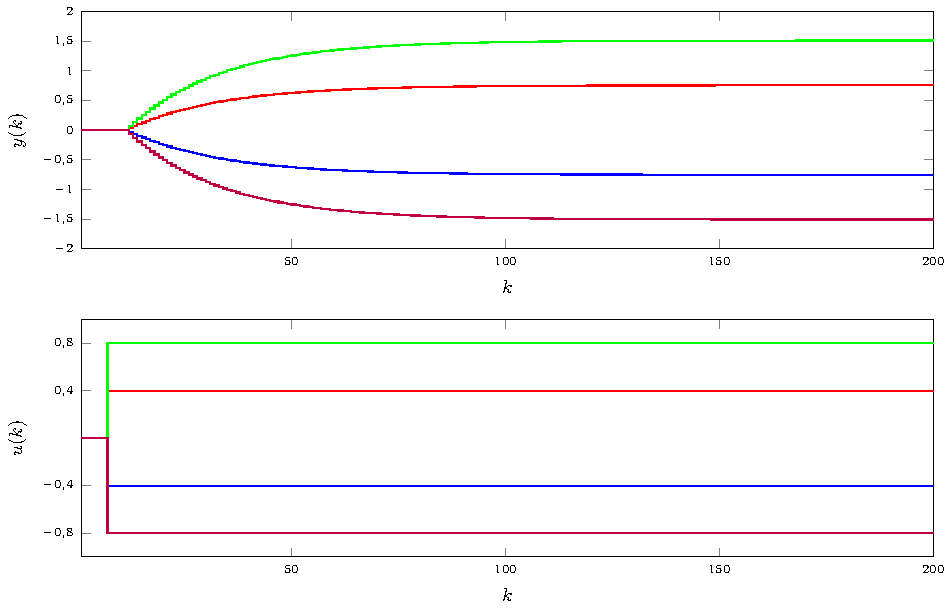
\includegraphics[scale=1]{../wykresy_pdf/odp_skok_ster.pdf}
\caption {Odpowied� skokowa toru wej�cie-wyj�cie}
\label{odp_skok_u}
\end{figure}

\begin{figure}[b]
\centering
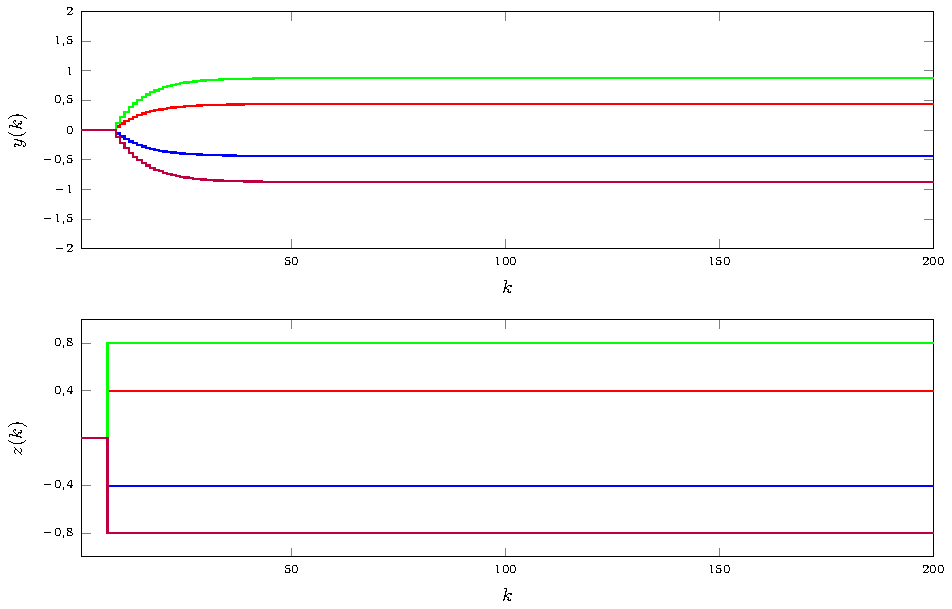
\includegraphics[scale=1]{../wykresy_pdf/odp_skok_zakl.pdf}
\caption {Odpowied� skokowa toru zak��cenie-wyj�cie}
\label{odp_skok_z}
\end{figure}

Charakterystyk� statyczn� $ y(u,z) $ procesu przedstawia wykres ~\ref{char_stat}

\begin{figure}[b]
\centering
\includegraphics[scale=1]{../wykresy_pdf/char_stat.pdf}
\caption {Charakterystyka statyczna procesu}
\label{char_stat}
\end{figure}

Z charakterystyki wida�, �e w�a�ciwo�ci statyczne procesu s� liniowe. W�a�ciwo�ci dynamiczne r�wnie�, st�d mo�emy obliczy� wzmocnienie statyczne toru wej�cie-wyj�cie:
$$ K = \frac{\Delta y}{\Delta u} = \num{1.8737} $$
oraz wzmocnienie statyczne toru zak��cenie-wyj�cie:
$$ K = \frac{\Delta y}{\Delta z} = \num{1.0837} $$